% Crucial Preamble
\documentclass[12pt,letterpaper]{article} \usepackage{amsmath} \usepackage{graphicx} \usepackage[margin=1in]{geometry} \usepackage{longtable}  \usepackage{amssymb}

% Extra Preamble
\usepackage{fancyhdr} \usepackage{enumitem} \usepackage{float} \usepackage{soul}
\usepackage{multicol} \usepackage[compact]{titlesec}


% frames with display breaks
\usepackage{mdframed}
\allowdisplaybreaks

% change spacing
\usepackage{setspace}
\setlength{\parskip}{0.4\baselineskip}

% Remove paragraph indentation
\setlength{\parindent}{0pt}

% Reduce space before and after section headings
%\titlespacing*{\section}{0pt}{0.1\baselineskip}{0.2\baselineskip}

% changes font
%\renewcommand{\familydefault}{\sfdefault}

% adds header and footer
\pagestyle{fancy}
\fancyhead{} \fancyhead[C]{CSI 2110 Cheat Sheet} \fancyhead[L]{CSI2110} \fancyhead[R]{Owen Daigle}
\fancyfoot{} \fancyfoot[C]{\thepage}


\begin{document}
	
	\begin{center}
		\Large\textbf{CSI 2110 Cheat Sheet} \\
		\vspace{0.5em}
	\end{center}
	
	\section{Analysis}
	We analyse algorithmns using the Big Oh notation. 
	
	A big Oh of O(n) means that the worst case running time of the algorithm is n.
	
	We say f(n) is O(g(n)) if there exist positive constants $n_0$ and c such that $f(n)\le cg(n) \forall n\ge n_0$.
	
	\begin{mdframed}
		\textbf{Ex. } Prove the following: 
		
		1. $2n^2 + 10n^3$ is O$(n^3)$
		We need to find the constants c and n0. 
		\begin{align*}
			2n^2 + 10n^3 \le 2n^3 + 10n^3 \le 12n^3 \implies c=12, n_0 = 1
		\end{align*}
		Since the constants exist, then it is proven.
	\end{mdframed}

	Big Omega is similar but it is the best case running time. 
	
	Big theta is the exact time. An algorithm of $\Theta(n)$ ALWAYS takes n time.
	
	\section{Stacks}
	A stack is a first in last out data type.
	
	We can \verb|push()|, \verb|pop()| to add or remove to the top of the stack. There is also \verb|isEmpty()|, \verb|pek()| (returns but does not remove the top) and \verb|size()|.
	
	\section{Queues}
	Queues are first in first out data types. 
	
	Elements are \textit{enqueued} at the read, and \textit{dequeued} from the front. 
	
	This can be inplemented using a \textbf{circular array, or a linkedlist}. 
	
	\section{Deques}
	A double ended queue (Deque) can be inserted at the front or rear of the queue, and can also be removed at the front or end of the queue. 
	
	A\textbf{ doubly linked list} works well for this. 
	
	\section{Lists/Sequence}
	This is a collection of elements in linear order. 
	
	\subsection{Array List}
	An array list can get from any index \verb|get(i)|, set any index \verb|set(i,e)|, add at any index \verb|add(i,e)|, or remove at any index \verb|remove(i)|.
	
	We want to implement the array lists using an\textbf{ extendable array} (double or increment the size when it gets full)
	
	\subsection{Positional List}
	
	A positional list is a list where we can get the previous or next element given a certain element in the list \verb|addBefore(p,e)|, \verb|addAfter(p,e)|. We can also add first or last \verb|addFirst()|, \verb|addLast()|.
	
	We implement positional lists using \textbf{linked lists}. 
	
	\subsection{Sequence}
	
	This provides all operations from the positional list and array list and has bridge methods as well such as \verb|atIndex(i)| (returns position), \verb|indexOf(p)| (returns index).
	
	This can be implemented using arrays or linked lists. 
	
	With \textbf{arrays}, the index based ops will be fast, but the positional ones will be slow. 
	
	With \textbf{linked lists}, the positional ops will be fast, but the index ones will be slow. 
	
	\section{Priority Queues}
	A priority queue is a queue where each element has a priority (key value pair). 
	
	We can \verb|insert(k,v)| in any order, and we can \verb|removeMin()| or just view \verb|min()|.
	
	If we use a \textbf{sorted sequence}, inserting takes O(n), and removing is O(1). 
	
	If we use an\textbf{ unsorted sequence}, inserting takes O(1), and removing is O(n).
	
	\subsection{Heaps}
	A Heap is a \textbf{complete} binary tree that stores a collection of key value pairs. 
	
	We can do either a \textbf{min heap} (min at top), or a \textbf{max heap} (max at top).
	
	With the min heap, the parent of a node is always greater than the children. 
	
	We implement these using a \textbf{priority queue}. 
	
	To remove from a heap, we remove the top element, then take from the bottom. Then we need to \textbf{downheap }until the heap is fixed. (Downheaping means swap with smallest child until child is bigger)
	
	To add on, we add at the first empty spot at the bottom, and then \textbf{upheap}. (Upheaping means swap with parent until parent is smaller).
	
	\subsection{Heap Construction}
	We use bottom up heap construction to build a heap. This takes O(n).
	
	For this, we start at \textbf{bottom right of heap}, then do a downheap on that parent. Then we go to the right and do it again. When that level is done, go up a level starting on the right. We will end up downheaping each element.  

	
	\section{Maps}
	A map stores and retrieves data based on a \textbf{unique key}. We have \verb|get(k)|, \verb|put(k,v)|, \verb|remove(k)|.
	
	A \textbf{sorted map} also has \verb|firstEntry()|, \verb|lastEntry()|.
	
	We can use an \textbf{ordered sequence} where searching takes O(logn), and inserting/removing take O(n).
	
	We can also use a \textit{better} \textbf{BST} (ideally a balanced one such as AVL) where the worst case search is O(n), but best case is O(logn). Inserting and deleting also depend on search so they are the same.
	
	\section{Trees}
	A tree has \textbf{internal nodes }(nodes with at least 1 child) and \textbf{external nodes }or Leafs (node without children).
	
	A tree is called \textit{binary} if each node has at most 2 children.
	
	We can traverse a binary tree using preorder, inorder, or postorder:
	\begin{enumerate}[noitemsep]
		\item Preorder means visit Root, then Left, then Right
		\item Inorder means visit Left, then Root, then Right
		\item Postorder means visit Left, then Right, then Root
	\end{enumerate}

	A binary tree is called \textbf{full} if each internal node has exactly 2 children.
	
	A binary tree of height h is called \textbf{complete} if the tree of height h-1 is perfect, and the rest of the nodes are added starting on the left.
	\begin{center}
		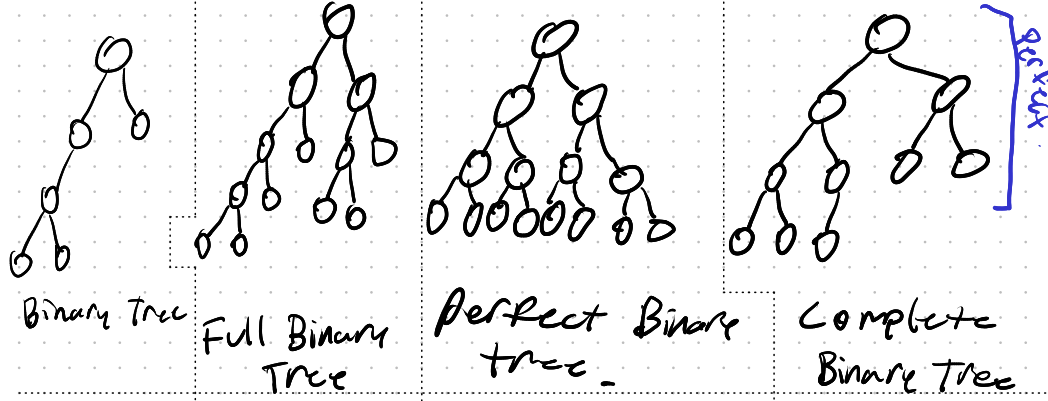
\includegraphics[width=0.8\linewidth]{trees}
	\end{center}

	We have some statistics about a full binary tree: 
	
	n is number of nodes, e is number of external nodes, i is number of internal nodes.
	\begin{align*}
		e = i+1\qquad n=2e-1
	\end{align*}
	These do NOT apply to a general binary tree.
	
	\textbf{All operations have O(1) except search which depends on the height of the tree}
	
	\subsection{AVL}
	An AVL tree is a BST where each internal node's subtrees heights can differ by at most 1. This means the height is O(logn).
	
	To insert or delete, we do the same thing as with a BST, except if any change renders the tree unbalanced, we need to rebalance the tree. 
	
	To rebalance, we go to the first node (from the bottom) that is unbalanced, then we do the inorder traversal from it down to the longest side naming the first node visited a, then b, then c. Then we align abc like this with their corresponding subtrees. 
	\begin{center}
		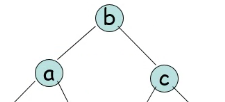
\includegraphics[width=0.2\linewidth]{abdc}
	\end{center}

	\begin{mdframed}[]
	\textbf{Ex. } Remove 7 from this tree.
	\begin{center}
		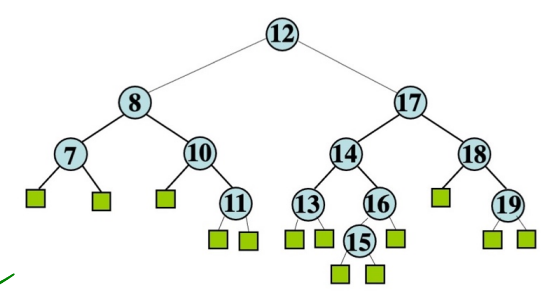
\includegraphics[width=0.4\linewidth]{ex}
	\end{center}
	When removing 7, we see that the 8 is unbalanced. So we do inorder traversal of it and its longest side (10, 11). We assign 8a, 10b, 11c.
	
	So we rearrange like:
	\begin{center}
		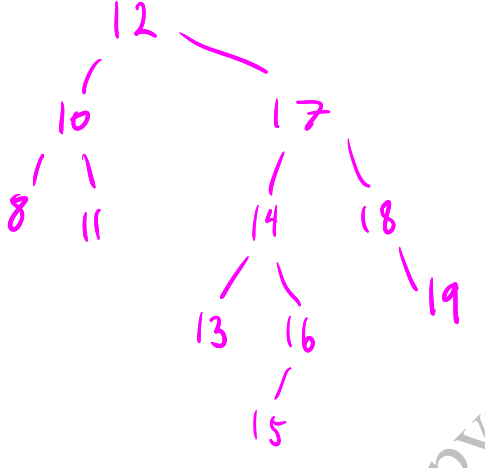
\includegraphics[width=0.3\linewidth]{ex2}
	\end{center}
	It is still unbalanced at the 12 node. So we do the inorder traversal there down the longest branch (ending with 15)
	
	12a, 14b, 17c
	\begin{center}
		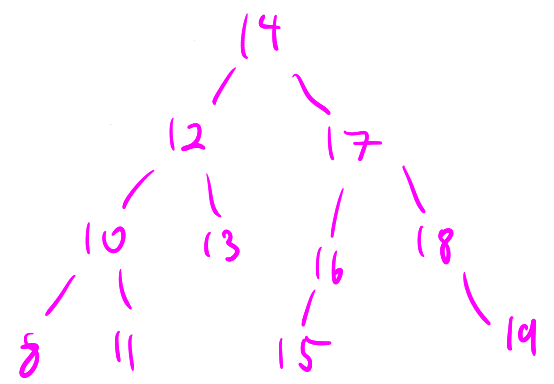
\includegraphics[width=0.3\linewidth]{ex3}
	\end{center}
	Now we are done. The tree is balanced. 	
	
	\end{mdframed}
	
	\subsection{2-4 Trees}
	A 2-4 tree is a non binary search tree where each node has 2, 3, or 4 children (and therefore 1, 2, or 3 keys) and all external nodes have the same depth. 
	
	When we insert, we go down the tree to find where in the key should go. If this causes 5 keys in a node, we split (usually using the third key which gets sent to the parent).
	
	When we delete, we remove the item to delete and replace with inorder successor. If this causes an underflow, we borrow from the parent and fuse the two children together or if the sibling has extra, we take from the sibling, put into the parent, and then steal from the parent. 
	
	\section{Hash Maps}
	We take a problem using a very large table, and use a function to map all data points to a smaller table. 
	
	To resolve collisions, we have a few methods:
	\begin{enumerate}[noitemsep]
		\item Chaining is creating a linked list at each spot in the hash table with items with duplicate hashes.
		\item Linear probing is we will go to the next empty spot linearly (h+0, h+1, h+2, h+3).
		\item Quadratic probing will go to the next spot squared (h+0, h+1, h+4, h+9)
		\item Double Hashing means we have a second hash function that we apply (h(k)+0d(k), h(k)+1d(k), h(k)+2d(k) for $h_j(k)=[h(k)+j^2d(k)]mod N$
	\end{enumerate}

	When we are using any of the methods 2-4, and we delete an item, we cannot just delete the item since we need a record that there was an item there. So we change it to AVAILABLE. This means not to stop searching for a key (since the key could be further along), but we can put a new key there.
	
	\section{Graphs}
	A graph has a set V of all vertices, and a set E of pairs of vertices called edges.
	
	We know that:
	\begin{align*}
		\sum deg(v) = 2m
	\end{align*}
	where m is the number of edges, n is number of vertices, and the degree of vertex v is the number of edges coming out of it. 
	
	A graph is connected if one can get from any vertex to any other vertex along the edges. Basically the graph does not have multiple isolated parts. 
	
	\subsection{DFS}
	
	\subsection{BFS}
	
	\subsection{Shortest Path}
	
	\subsection{MST}
	
	\section{Sort}
	
	\subsection{Mergesort}
	
	\subsection{Quicksort}
	
	\subsection{Bucket Sort}
	
	\subsection{Radix Sort}
	
	\subsection{Quadratic Sorts}
	
	
	
	
	
	
	
\end{document}